
\section{结果与分析}

\subsection{模型预测结果分析}

对于CNN,训练过程的可视化数据如\ref{fig4-1}所示,该网络在MNIST训练集下在第一个epoch就可以收敛地不错,之后训练集准确度保持在0.990左右,验证集准确度在0.987左右,基本符合CNN训练MNIST训练集的情况。

\begin{figure}[h!]
    \centering
    \includesvg[width=0.7\textwidth]{figure/train.svg}
    \caption{训练中损失,训练集准确度和验证集准确度}
    \label{fig4-1}
\end{figure}

对于CNN预测分类的混淆矩阵如\ref{fig4-2},从矩阵中分析,发现CNN网络对于‘5’、‘6’、‘9’的识别能力稍差,总体来看识别比较准确。

\begin{figure}[h!]
    \centering
    \includesvg[width=0.55\textwidth]{figure/confuse.svg}
    \caption{混淆矩阵}
    \label{fig4-2}
\end{figure}

对于KNN和CNN两个模型,准确度,召回率,F1值的表格如下\ref{table4-1},可以看到,在各个评判标准下,KNN的都略逊色于CNN网络,这是因为CNN卷积的特性非常适合拿来做图像处理,且模型复杂,表达能力更强。

\begin{table}[h]
    \caption{\textbf{准确度,召回率,F1值}}
    \label{table4-1}
    \centering
    \begin{tabularx}{\linewidth}{XXXXX}
        \toprule 
        \textbf{模型}       &   \textbf{准确度}     & \textbf{召回率}   &   \textbf{F1} \\
        \midrule 
        CNN           &   98.864\%     &   98.859\%    &    98.858\% \\
        KNN           &   94.952\%     &   94.925\%    &    94.921\% \\
        \bottomrule
    \end{tabularx}
\end{table}

\subsection{与现有模型对比}

我在kaggle上分别上传了CNN、KNN和预训练的Resnet50模型训练后的预测,成绩如图\ref{fig4-3}所示,submission1, 2, 3分别对应ResNet50, CNN, KNN的预测成绩。

\begin{figure}[h!]
    \centering
    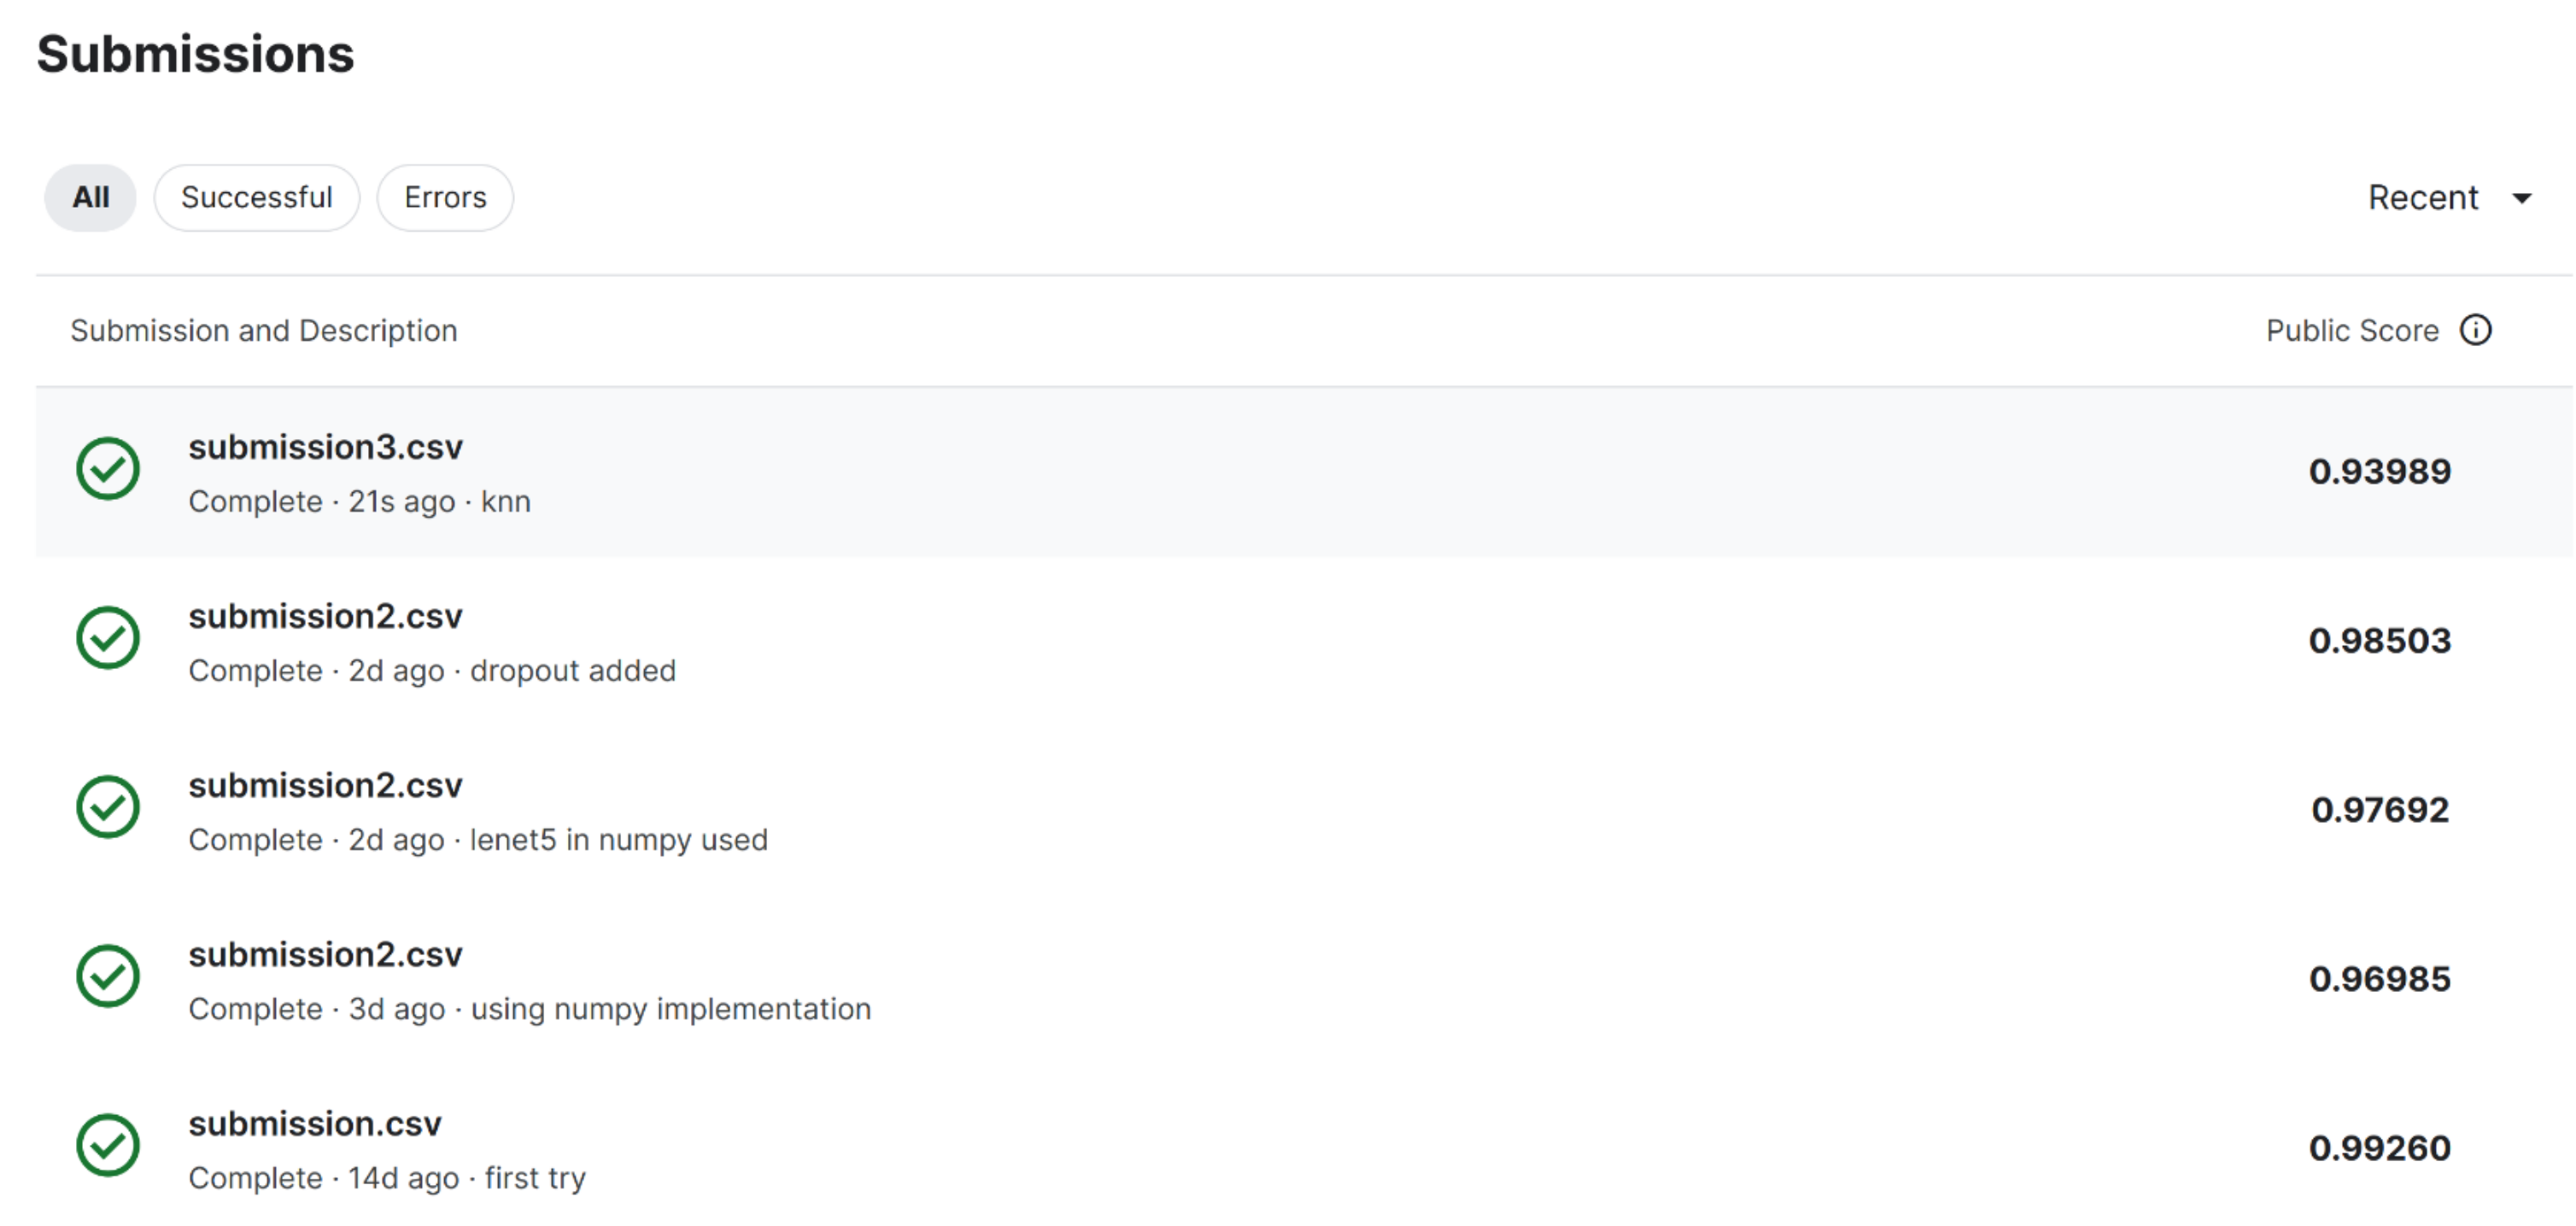
\includegraphics[width=0.7\textwidth]{figure/kaggle.png}
    \caption{kaggle分数}
    \label{fig4-3}
\end{figure}

可以看到Resnet作为深度卷积神经网络,在没有大量调参的情况下依然比其余两个numpy实现的模型效果要好上不少,而CNN也是卷积神经网络,结果比KNN要好。当然由于KNN网络的性质,如果训练得当可以在kaggle上做到全对,accuracy达到1。

\subsection{优化方向}

对于CNN网络,现有的优化方向有几条,可以改进优化器,使用Adam优化器进行梯度下降,也可以加深神经网络,采用使用新的层例如BN层(batch normalization),使用块(VGG),进行预训练等方法。